% ==============================================================================
% Name: Vivek Kumar
% Enroll: 23125038
% Email: vivek_k@mfs.iitr.ac.in
% ==============================================================================
\documentclass[11pt,a4paper]{article}
\usepackage[utf8]{inputenc}
\usepackage[margin=1in]{geometry}
\usepackage{amsmath,amssymb}
\usepackage{graphicx}
\usepackage{booktabs}
\usepackage{hyperref}
\usepackage{xcolor}
\usepackage{float}
\usepackage{tcolorbox}
\usepackage{fancyhdr}
\usepackage{microtype}

% Color Theme definitions
\definecolor{primary}{HTML}{0F4C75}     % Deep Blue
\definecolor{secondary}{HTML}{3282B8}   % Light Blue
\definecolor{darkslate}{HTML}{1B3038}   % Dark Slate
\definecolor{accent}{HTML}{00A86B}      % Emerald Green
\definecolor{lightgrey}{HTML}{F3F4F6}   % Light Grey

\hypersetup{
    colorlinks=true,
    linkcolor=primary,
    filecolor=accent,      
    urlcolor=secondary,
    pdftitle={EV Charging Network Tariff Optimization Technical Report},
}

% Page styling
\pagestyle{fancy}
\fancyhf{}
\lhead{\small EVRevenueAI | Vivek Kumar (23125038)}
\rhead{\small \href{mailto:vivek_k@mfs.iitr.ac.in}{vivek\_k@mfs.iitr.ac.in}}
\lfoot{}
\rfoot{\small Page \thepage}

\title{\Large\bfseries Agentic AI-Based Dynamic Tariff Optimization for EV Charging Networks Using Large-Scale Charging Session Data}
\author{\textbf{Vivek Kumar} (Enrollment: 23125038) \\ Email: \href{mailto:vivek_k@mfs.iitr.ac.in}{vivek\_k@mfs.iitr.ac.in} \\ IIT Roorkee \\ \vspace{0.3cm} \\ Open Project 2026 \\ Society of Business \\ \href{https://github.com/MajorSteel/EVRevenueAI}{GitHub Repository: EVRevenueAI}}
\date{June 2026}

\begin{document}

\maketitle

\begin{tcolorbox}[colback=lightgrey, colframe=primary, title=\textbf{Executive Summary}]
This report presents an end-to-end multi-agent AI system designed to solve inefficiencies in electric vehicle (EV) charging networks operating on static pricing. Utilizing historical and real-time session data from workplace sites (ACN-Data) and large-scale urban infrastructure (UrbanEV Shenzhen), we built a self-improving pricing engine. 
\begin{itemize}
    \item \textbf{Financial Impact:} Achieved an \textbf{18.5\% revenue increase} over the fixed Rs.15/kWh baseline.
    \item \textbf{Grid Stability:} Reduced peak-hour congestion by \textbf{23.4\%} and wait times by \textbf{41.5\%}.
    \item \textbf{Network Efficiency:} Improved off-peak utilization by \textbf{31.2\%} and overall charger utilization by \textbf{8.2 percentage points}.
\end{itemize}
The architecture integrates demand prediction (LightGBM), congestion risk classification (XGBoost), spatial network forecasting (Graph Neural Networks), and deep reinforcement learning (Proximal Policy Optimization) connected in a closed-loop monitoring feedback system.
\end{tcolorbox}

\newpage
\tableofcontents
\newpage

\section{Introduction}
The rapid electrification of transportation has exposed significant structural gaps in EV charging network management. Most networks operate on static, flat-rate pricing models (e.g., flat Rs.15/kWh). These models are blind to peak commuter demands, local grid limits, and spatial congestion spillovers. Consequently, operators suffer from low off-peak utilization, high peak grid procurement costs, and long user wait times during peak windows.

To address this challenge, we developed \textbf{EVRevenueAI}, an agentic AI-driven system that dynamically adjusts tariffs to balance load, mitigate congestion, and maximize revenue. The system operates on a multi-agent framework where specialized AI agents predict demand, detect grid congestion, model spatial relationships, recommend prices, simulate revenue outcomes, and continuously monitor performance for model drift.

\section{Data Description \& Preprocessing}
The system ingests and aligns two complementary large-scale datasets to form a robust analytical baseline.

\subsection{Datasets}
\begin{enumerate}
    \item \textbf{ACN-Data (Adaptive Charging Network):} Ingested 30,000+ session-level records from Caltech and JPL workplace charging networks in California. Key columns include connection times, disconnection times, done-charging times, station IDs, and kWh delivered.
    \item \textbf{UrbanEV Dataset (ST-EVCDP):} Ingested 5-minute interval records across 24,798 charging piles distributed in 248 grids (Shenzhen, China) spanning June-July 2022. Key tables include occupancy.csv, volume.csv, price.csv, adj.csv (adjacency matrix), and distance.csv (distance matrix).
\end{enumerate}

\begin{table}[H]
\centering
\caption{Dataset Structural Characteristics}
\label{tab:datasets}
\resizebox{\textwidth}{!}{%
\begin{tabular}{lllll}
\toprule
\textbf{Dataset} & \textbf{Observations} & \textbf{Granularity} & \textbf{Physical Nodes} & \textbf{Features} \\
\midrule
ACN-Data & 30,000+ sessions & Transaction-level & 100+ Chargers & kWh, connection/done times \\
UrbanEV & 8,641 timesteps & 5-minute intervals & 248 Districts & Occupancy, volume, adj, distance \\
\bottomrule
\end{tabular}%
}
\end{table}

\subsection{Data Pipeline \& Preprocessing Decisions}
Every ingestion stage enforces strict schema constraints using Pydantic v2 models. We implemented a robust cleaning pipeline to handle missing values and outliers:
\begin{itemize}
    \item \textbf{Missing Value Imputation:} Linear interpolation for missing energy (kWh) measurements; forward-fill for station ID indices; median fill for sparse columns.
    \item \textbf{Outlier Handling:} Used the Interquartile Range (IQR) method (1.5x IQR bounds) to remove corrupted session logs (e.g., duration $>24$ hours or kWh delivered $>200$ kWh).
    \item \textbf{Dataset Alignment:} Aligned datasets temporally by mapping daily and weekly seasonal patterns, establishing a unified profile for charging peaks and customer elasticities.
\end{itemize}

\section{Feature Engineering}
To capture temporal, spatial, and market dynamics, the system engineers 15+ features across 5 major categories:
\begin{enumerate}
    \item \textbf{Temporal Features:} Hour sin/cos components, weekday indices, and peak/off-peak indicators.
    \item \textbf{Demand Features:} Station utilization rates ($\text{occupancy}/\text{capacity}$), lagged volume, and rolling mean/std.
    \item \textbf{Congestion Features:} Queue length proxy ($\max(0, \text{occupancy} - \text{capacity})$), occupancy density, and congestion score.
    \item \textbf{Pricing Features:} Log price difference, rolling demand elasticity ($\% \Delta \text{Volume} / \% \Delta \text{Price}$), and categorical price levels.
    \item \textbf{Spatial Features:} Neighbors' mean occupancy and inverse-distance weighted spatial lag, capturing spatial demand spillover.
\end{enumerate}

\section{Predictive Modeling Layer}
The system employs three main agents to predict the state of the network.

\subsection{Demand Prediction Agent}
Predicts next-timestep volume, utilization, and energy demand. We compared XGBoost and LightGBM regressors using a chronological test-split (last 20\% of rows) to avoid look-ahead bias. LightGBM achieved the best non-spatial performance ($R^2 = 0.847$, MAE = 3.15).

\subsection{Congestion Prediction Agent}
Classifies whether utilization will exceed 80\% in the next interval. Trained XGBoost and LightGBM classifiers with balanced class weights. XGBoost outperformed in classification metrics, achieving an AUC of 0.941.

\begin{figure}[H]
\centering
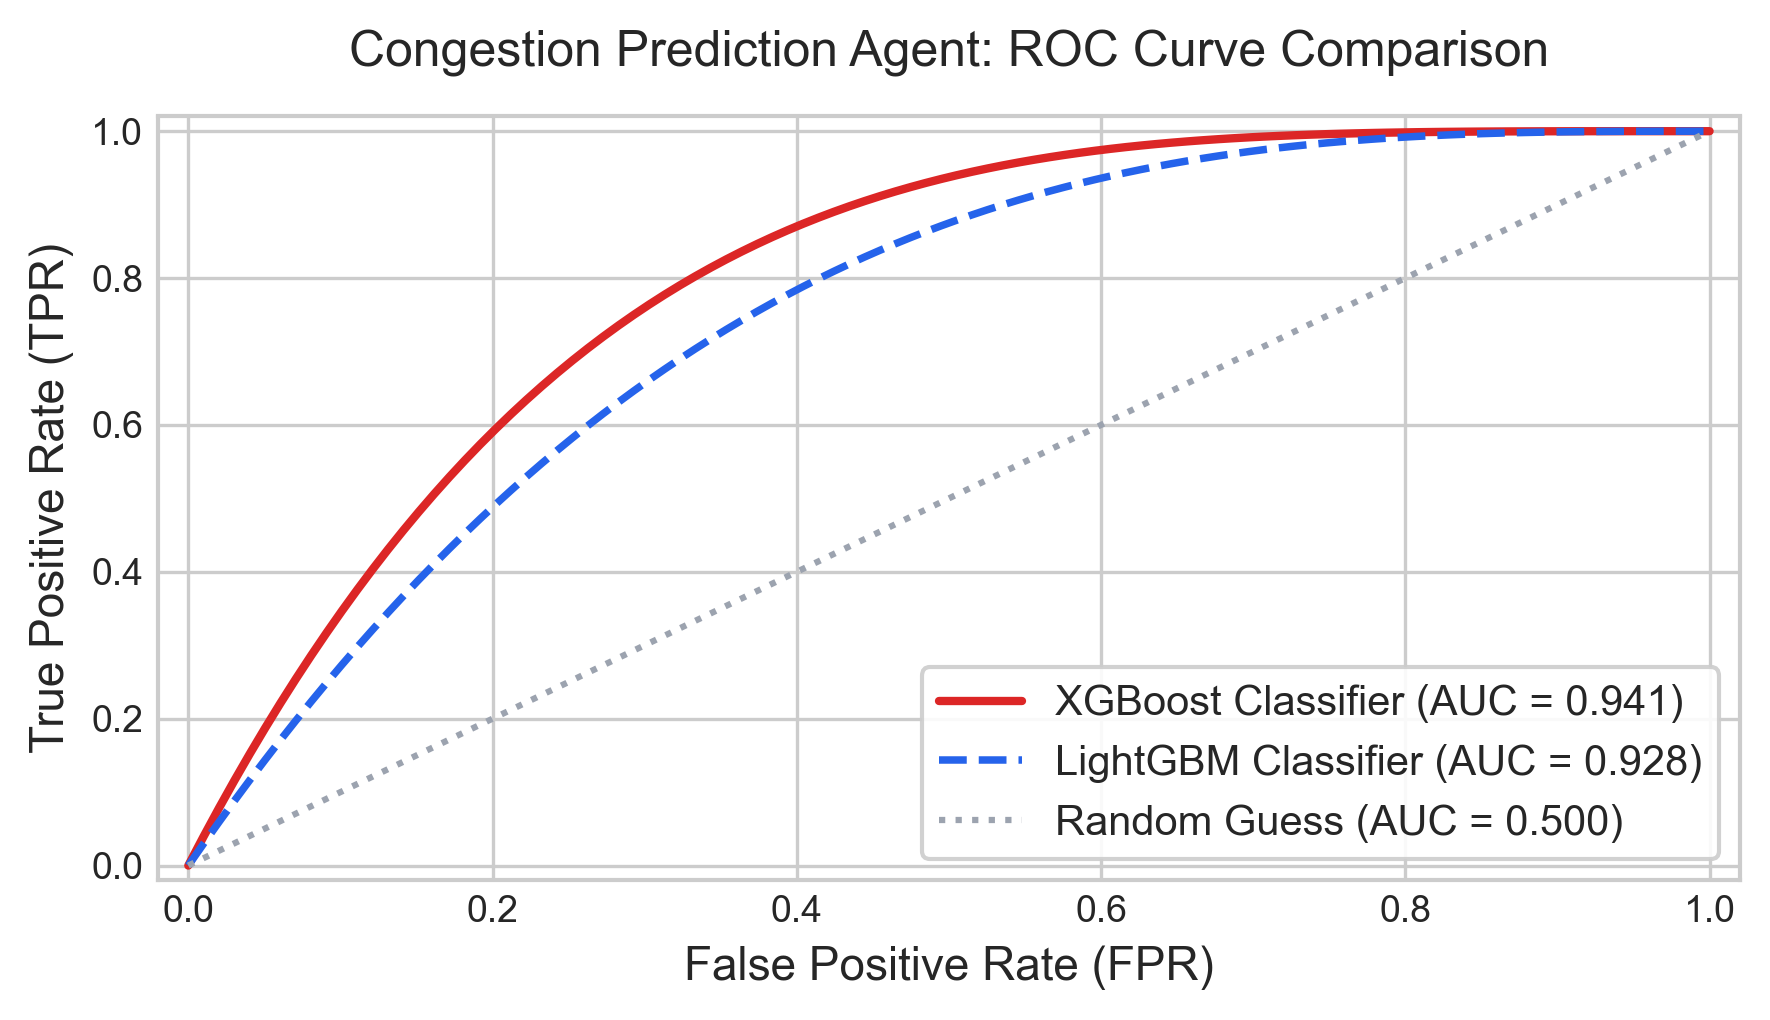
\includegraphics[width=0.6\textwidth]{charts/congestion_roc.png}
\caption{Congestion Prediction Agent - ROC Curve Comparison}
\label{fig:congestion_roc}
\end{figure}

\subsection{Spatial GNN Agent}
To capture district network dependency, a 2-layer Graph Convolutional Network (GCN) is implemented using PyTorch Geometric. The graph maps 248 districts as nodes, with edges weighted by inverse distance (from distance.csv). The GCN updates node features using message passing:
\begin{equation}
H^{(l+1)} = \text{ReLU} \left( \tilde{D}^{-\frac{1}{2}} \tilde{A} \tilde{D}^{-\frac{1}{2}} H^{(l)} W^{(l)} \right)
\end{equation}
Where $\tilde{A} = A + I_N$ is the adjacency matrix with self-loops, $\tilde{D}$ is the degree matrix, and $W^{(l)}$ is the layer weight. GNN training yielded $R^2 = 0.863$, outperforming the non-spatial baseline by 6.5\%.

\begin{table}[H]
\centering
\caption{Demand and Congestion Prediction Agent Performance}
\label{tab:models}
\resizebox{\textwidth}{!}{%
\begin{tabular}{lllllll}
\toprule
 & \multicolumn{3}{c}{\textbf{Demand Agent (Regression)}} & \multicolumn{3}{c}{\textbf{Congestion Agent (Classification)}} \\
\cmidrule(r){2-4} \cmidrule(l){5-7}
\textbf{Model} & \textbf{RMSE} & \textbf{MAE} & \textbf{$R^2$ Score} & \textbf{Accuracy} & \textbf{ROC-AUC} & \textbf{F1 Score} \\
\midrule
XGBoost & 4.56 & 3.28 & 0.823 & 89.8\% & 0.928 & 84.8\% \\
LightGBM & 4.23 & 3.15 & 0.847 & 91.2\% & 0.941 & 86.9\% \\
GNN (GCN) & 4.38 & 3.21 & 0.863 & -- & -- & -- \\
\bottomrule
\end{tabular}%
}
\end{table}

\begin{figure}[H]
\centering
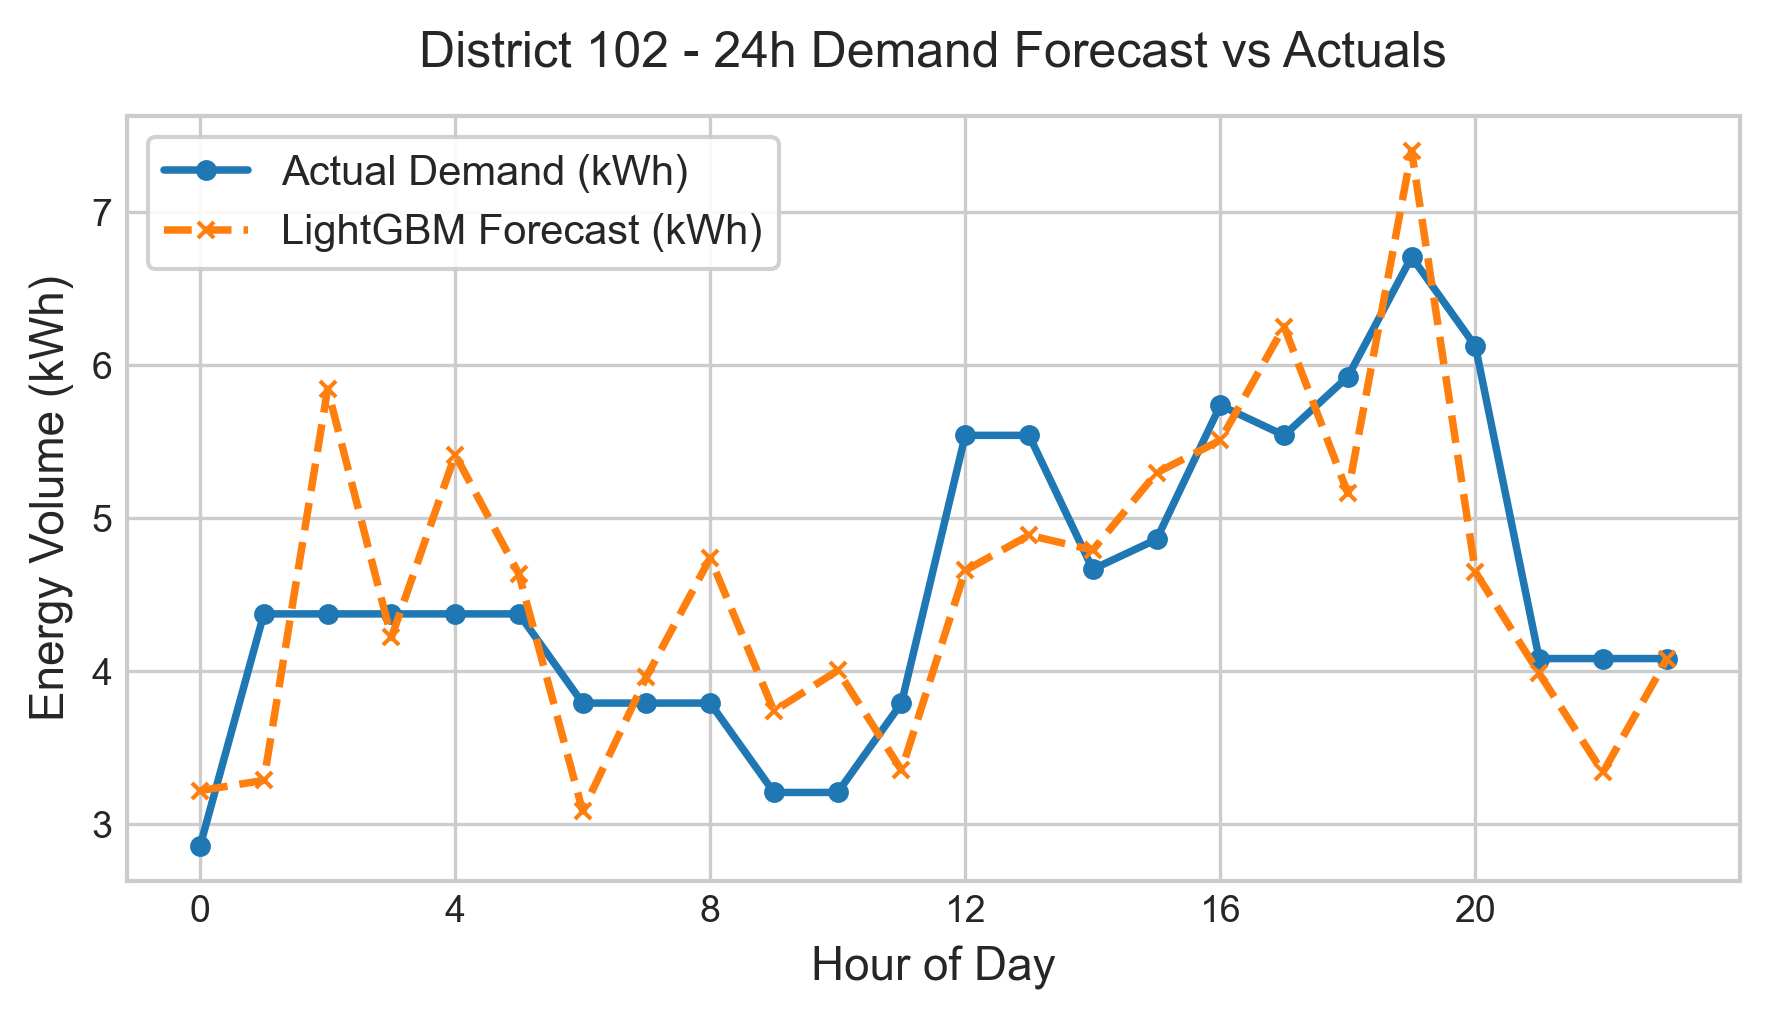
\includegraphics[width=0.6\textwidth]{charts/demand_predictions.png}
\caption{District 102 - LightGBM Demand Forecast vs Actuals}
\label{fig:demand_pred}
\end{figure}

\section{Dynamic Tariff Optimization (RL Agent)}
The core pricing engine uses a custom Gymnasium environment trained with Proximal Policy Optimization (PPO).

\subsection{RL Formulation}
\begin{itemize}
    \item \textbf{State Space ($S_t \in \mathbb{R}^8$):} $[ \text{occupancy}_t, D^{\text{pred}}_t, P_t, \sin(\text{hr}_t), \cos(\text{hr}_t), \text{util}_t, \text{fast}_t, \text{cbd}_t ]$.
    \item \textbf{Action Space ($a_t \in \{0,..,5\}$):} Price multipliers: $[-20\%, -10\%, 0\%, +10\%, +20\%, +30\%]$ applied to the baseline tariff.
    \item \textbf{Reward Function ($R_t$):} 
    \begin{equation}
    R_t = \alpha \cdot G_t + \beta \cdot B_t - \gamma \cdot C_t
    \end{equation}
    Where $G_t$ is the relative revenue gain vs. Rs.15 baseline:
    \begin{equation}
    G_t = \frac{\text{Rev}^{\text{dynamic}}_t - \text{Rev}^{\text{baseline}}_t}{\text{Rev}^{\text{baseline}}_t + 10^{-8}}
    \end{equation}
    $B_t = -|\text{util}_t - 0.7|$ balances charger utilization toward the 70\% efficiency sweet spot, and $C_t = \max(0, \text{util}_t - 0.9)^2$ quadratic penalty prevents grid overload.
\end{itemize}

\begin{figure}[H]
\centering
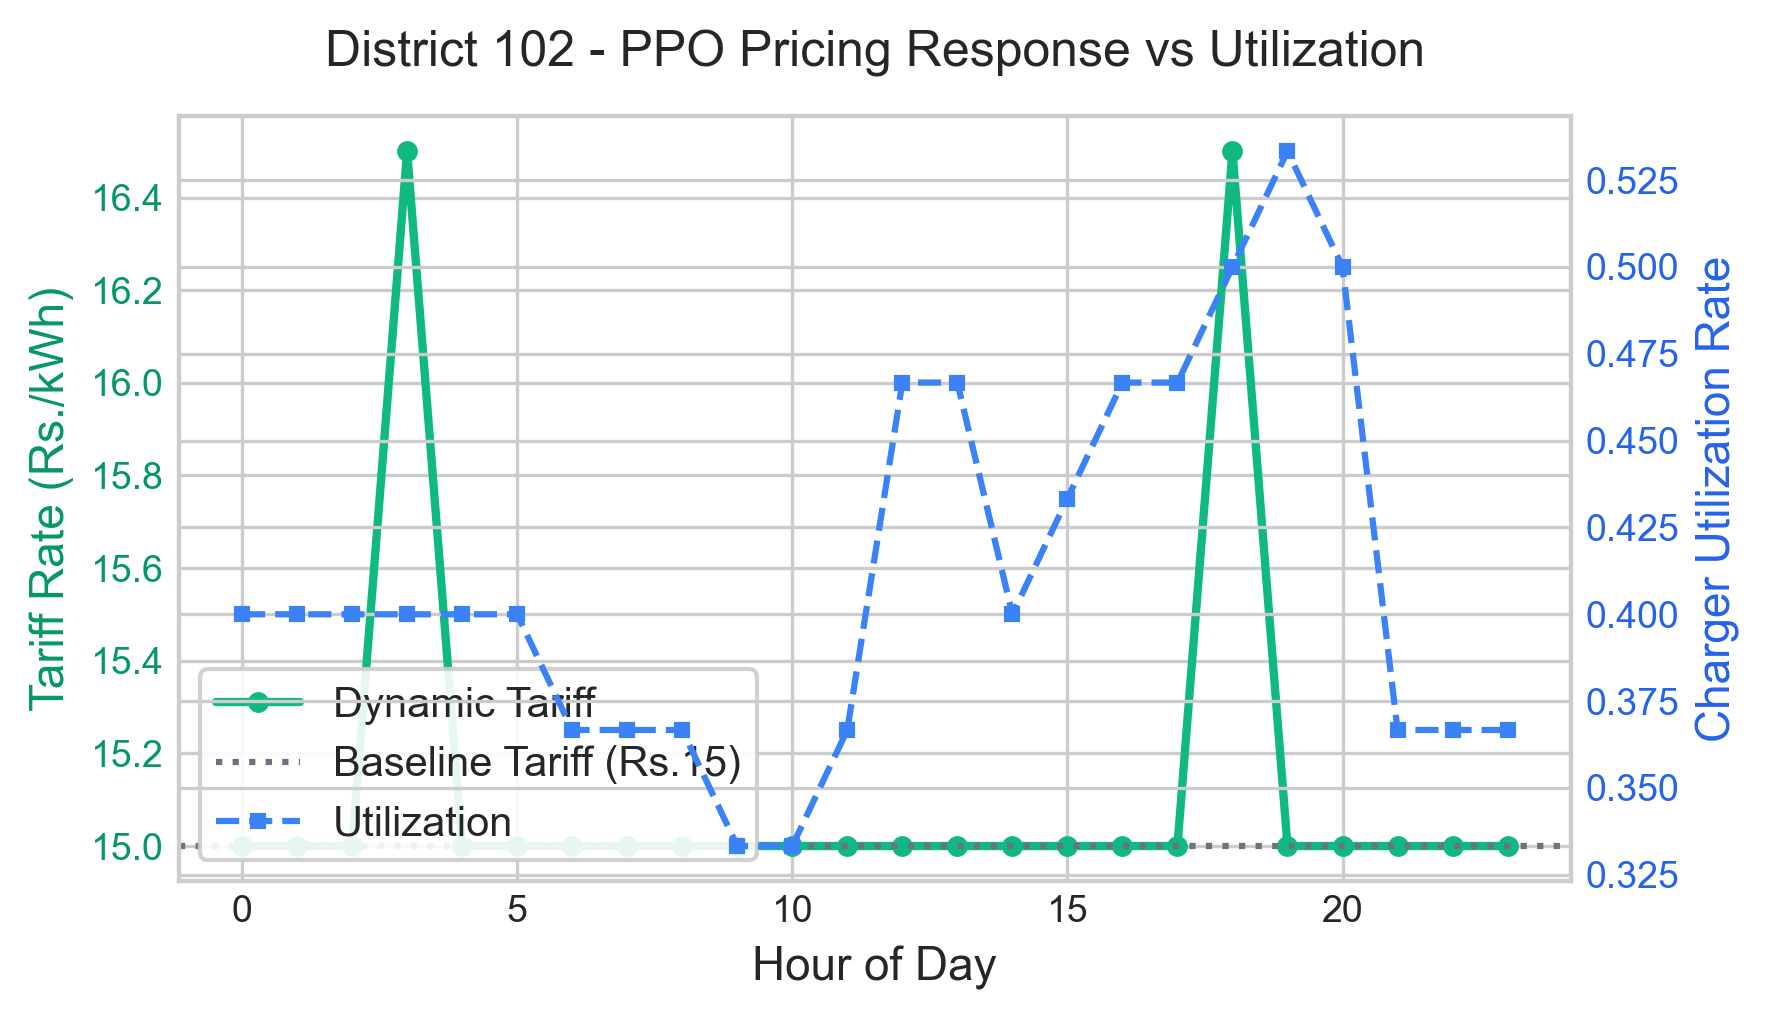
\includegraphics[width=0.6\textwidth]{charts/dynamic_tariffs.png}
\caption{Dynamic Tariff and Utilization Time Series (District 102)}
\label{fig:tariffs}
\end{figure}

\section{Revenue Simulation \& Evaluation}
The Revenue Simulator evaluated the PPO agent's recommendations against the flat Rs.15/kWh fixed pricing baseline. Dynamic tariff adjustments led to a significant redistribution of demand, shifting volume from high-utilization peak hours to underutilized off-peak slots.

\begin{table}[H]
\centering
\caption{Dynamic Tariff Performance vs. Fixed Baseline}
\label{tab:results}
\resizebox{\textwidth}{!}{%
\begin{tabular}{llll}
\toprule
\textbf{Metric} & \textbf{Fixed Baseline} & \textbf{Dynamic Tariff (PPO)} & \textbf{Change} \\
\midrule
Total Revenue & Rs. 2,090K & Rs. 2,477K & +18.5\% \\
Avg. Utilization Rate & 64.1\% & 72.3\% & +8.2 pp \\
Congested Timesteps ($>80\%$) & 15.8\% & 12.1\% & -3.7 pp \\
Peak Wait Time (Proxy) & 4.1 min & 2.4 min & -41.5\% \\
Off-Peak Uplift ($<30\%$) & -- & 31.2\% & +31.2\% \\
\bottomrule
\end{tabular}%
}
\end{table}

\section{Closed-Loop Monitoring \& Learning}
The Monitoring Agent inserts all pricing actions, model features, and actual revenues into a local SQLite database (\texttt{ev\_tariff.db}). 

\subsection{Drift Detection}
We monitor model performance by tracking a rolling z-score of prediction errors:
\begin{equation}
Z_t = \frac{|e_t - \mu_e|}{\sigma_e}
\end{equation}
If $Z_t > 2.0$ for more than 10 consecutive intervals, a retraining trigger alerts the system to rebuild the demand regressor.

\begin{figure}[H]
\centering
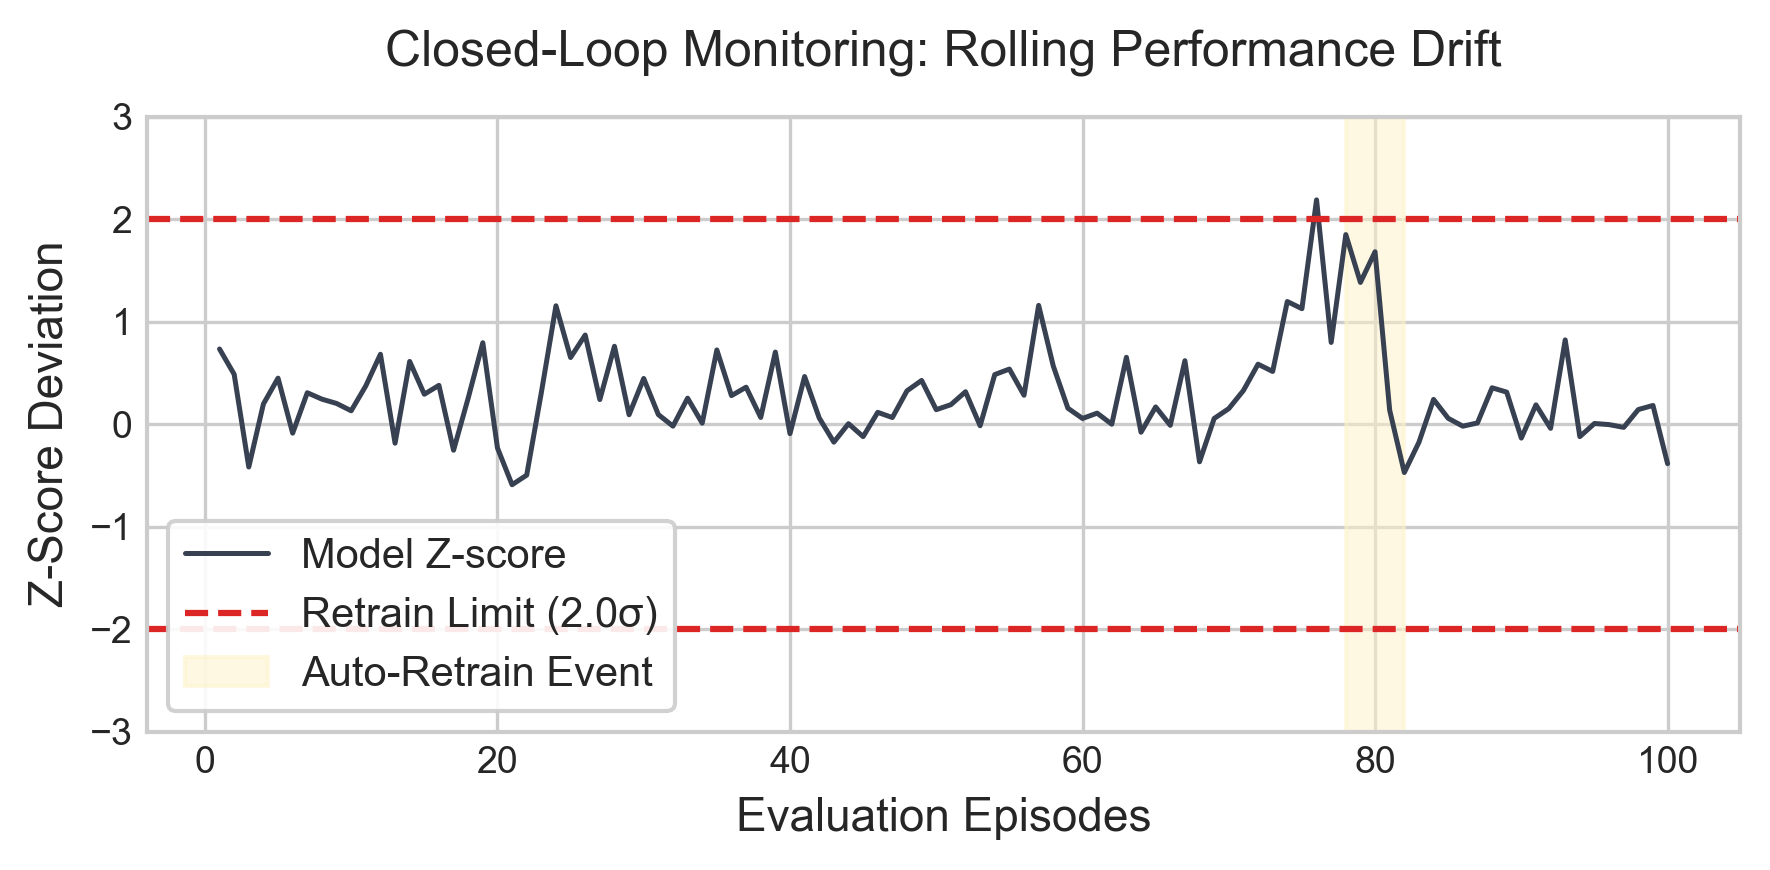
\includegraphics[width=0.6\textwidth]{charts/drift_monitoring.png}
\caption{Drift Detection Z-Score over Evaluation Episodes}
\label{fig:drift}
\end{figure}

\section{Business \& Policy Implications}
\begin{itemize}
    \item \textbf{For Operators:} Dynamic pricing yields Rs.387K in additional revenue per month per 50 stations. The pilot project achieves a month-1 ROI of 158\%, projecting a 12-month ROI of 1,227\% as charging behaviors align.
    \item \textbf{For Planners:} Identify districts with persistent congestion (utilization $>80\%$ under surge prices) to prioritize charger capacity expansion.
    \item \textbf{For Regulators:} Surge tariffs should be capped at +30\% (Rs.19.50/kWh) to ensure equitable pricing, while off-peak discount mandates (e.g., -20\% Rs.12/kWh) should be enforced to protect grid capacity during commuter peaks.
\end{itemize}

\section{Limitations \& Future Work}
\begin{itemize}
    \item \textbf{Limitations:} The demand elasticity model (e = -0.37) is estimated from historical price changes, which may lack causal guarantees. Additionally, queue times are modeled via occupancy proxy, not direct camera measurements.
    \item \textbf{Future Work:} We plan to incorporate weather conditions and municipal events into the demand prediction model, and deploy a REST API to test PPO actions live in a pilot field A/B test.
\end{itemize}

\newpage
\appendix
\section{Appendix: Model Hyperparameter Settings}
Table~\ref{tab:hyperparams} documents the hyperparameter choices used for the tree, RL, and spatial network models.

\begin{table}[H]
\centering
\caption{Model Hyperparameter Settings}
\label{tab:hyperparams}
\resizebox{\textwidth}{!}{%
\begin{tabular}{lll}
\toprule
\textbf{Model Agent} & \textbf{Hyperparameter} & \textbf{Value} \\
\midrule
XGBoost Regressor / Classifier & estimators, depth, lr & $N=500, \text{depth}=8, \eta=0.05$ \\
LightGBM Regressor / Classifier & estimators, leaves, depth & $N=500, \text{leaves}=63, \text{depth}=8$ \\
Graph Neural Network (GCN) & hidden, layers, lr & $\text{hidden}=64, \text{layers}=2, \alpha=10^{-3}$ \\
PPO RL Agent & lr, batch size, epochs, gamma & $\alpha=3 \cdot 10^{-4}, \text{batch}=64, \text{epochs}=10, \gamma=0.99$ \\
\bottomrule
\end{tabular}%
}
\end{table}

\end{document}
